\documentclass[11pt]{article}
\usepackage[margin=1in]{geometry}
\usepackage{amsmath,amssymb,amsthm}
\usepackage{graphicx}
\usepackage[hidelinks]{hyperref}
\usepackage{microtype}

\newtheorem{theorem}{Theorem}
\newtheorem{lemma}{Lemma}
\newcommand{\T}{\mathbb T}
\newcommand{\Z}{\mathbb Z}
\newcommand{\D}{\mathbb D}
\newcommand{\one}{\mathbf 1}

\title{Question 5.7 of arXiv:2507.00186:\\
all non-bounded-remainder intervals give weak mixing}
\author{Literature-implied solution packet}
\date{11 August 2026}

\begin{document}
\maketitle

\noindent\textbf{Status.}
\texttt{literature\_implied\_answer}; complete, in a stronger
all-irrational-rotation form.
The one-sided discrepancy theorem needed below is classical (Hal\'asz, 1976).
The application to the source paper's operator question is the identification
recorded in this packet; no claim of a new theorem is made.

\section{Source question}

The source is Valentin Gillet, \emph{Linear dynamics of random products of
operators}, arXiv:2507.00186v3, Question 5.7, printed/PDF page 45.  For an
irrational rotation $R_\alpha$, it takes
\[
 A_1=[0,b),\qquad A_2=[b,1),
\]
and asks whether Corollaries 3.22 and 3.23 remain true when
$b\notin \Z\alpha$ modulo one.  Those corollaries assert topological weak
mixing, almost surely in the starting point, for random products of adjoints
of multiplication operators satisfying either of the two analytic hypotheses
listed there.

\begin{center}
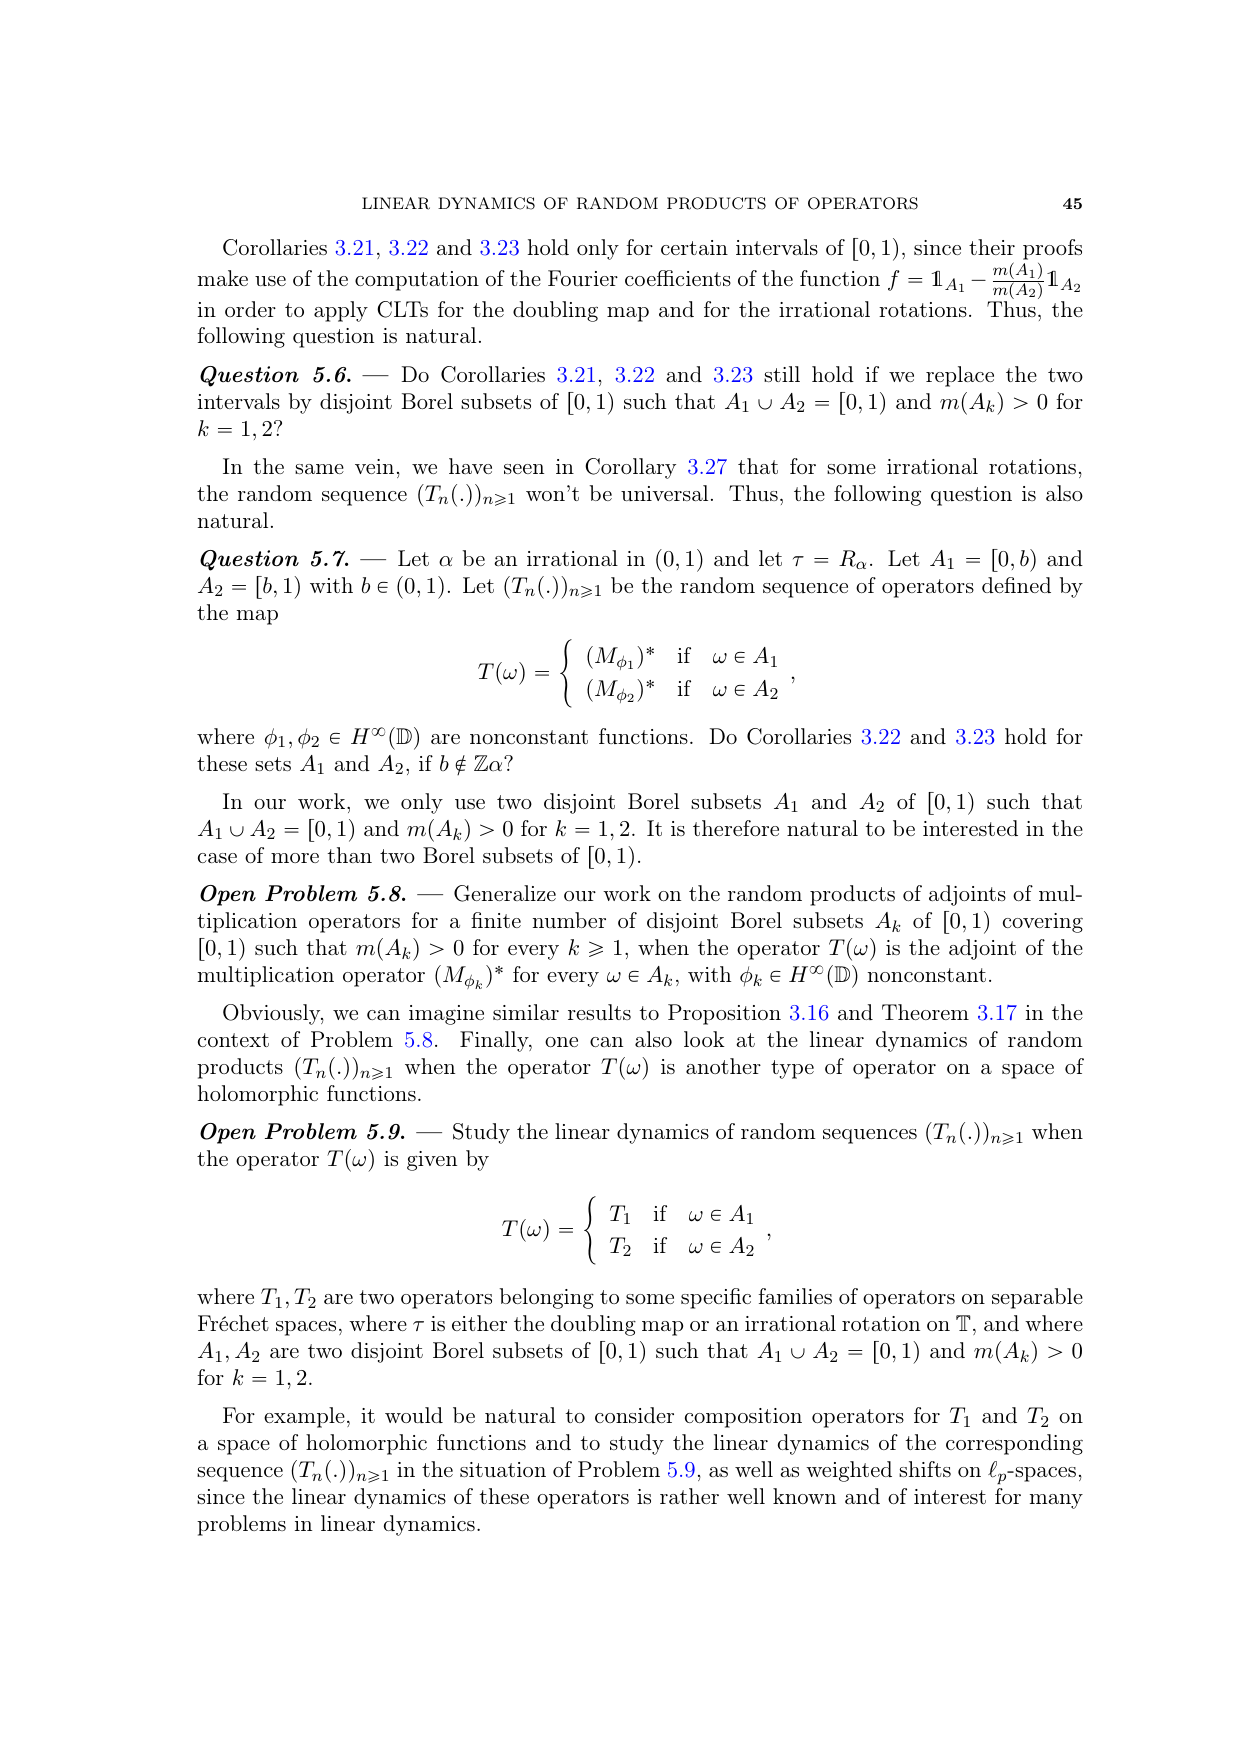
\includegraphics[width=.92\textwidth]{figures/open_question_page_45.png}
\end{center}

The relevant centered function is
\begin{equation}\label{eq:fsource}
 f=\one_{[0,b)}-\frac{b}{1-b}\one_{[b,1)}
   =\frac{1}{1-b}\bigl(\one_{[0,b)}-b\bigr).
\end{equation}
Theorems 3.19 and 3.20 of the source imply both requested corollaries as soon
as the Birkhoff sums of $f$ have limsup $+\infty$ and liminf $-\infty$ almost
everywhere.

\section{Classical one-sided input}

For an ergodic probability-preserving map $T$ and a measurable set $A$, write
\[
 \Delta_n(A;x)=\sum_{j=0}^{n-1}\bigl(\one_A(T^jx)-\mu(A)\bigr).
\]
Hal\'asz proved that if $\Delta_n(A;x)$ is bounded on one side in $n$ for
$x$ in a set of positive measure, then $e^{2\pi i\mu(A)}$ is an eigenvalue of
$T$.  S\'os's survey states this strengthening explicitly on printed page 234:

\begin{center}
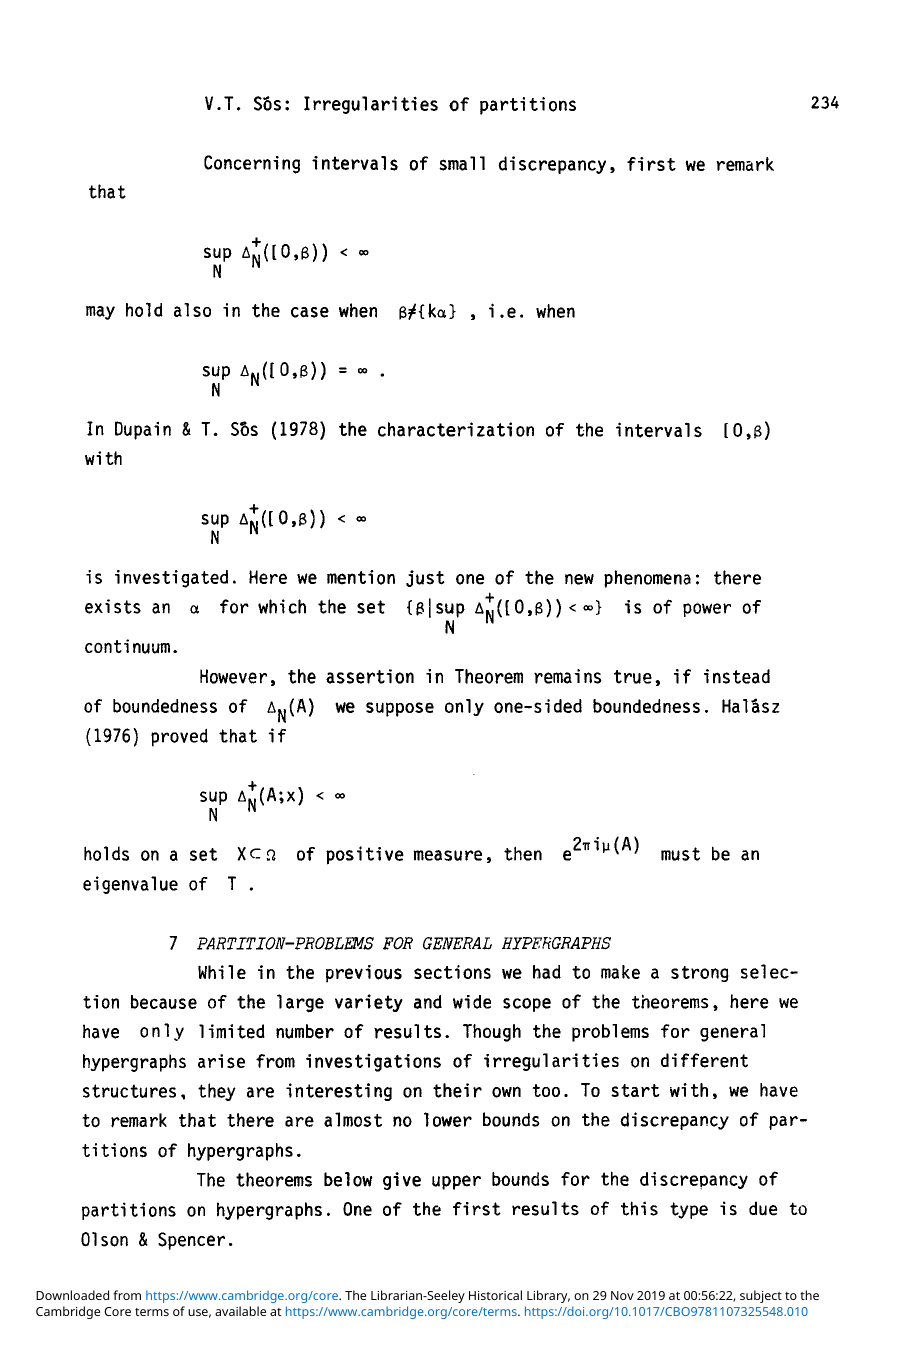
\includegraphics[width=.60\textwidth]{figures/halasz_one_sided_theorem_page_234.png}
\end{center}

For completeness, here is a short coboundary proof of the precise bridge used
in this packet.\par\medskip

\begin{lemma}[one-sided bounded sums force a measurable coboundary]
Let $T$ be an ergodic probability-preserving transformation and let
$g\in L^\infty$ be real with $\int g\,d\mu=0$.  If
$\inf_{n\geq 0}S_ng(x)>-\infty$ almost everywhere, where
$S_ng=\sum_{j=0}^{n-1}g\circ T^j$ and $S_0g=0$, then there is a finite
measurable $G\geq0$ such that
\[
 g=G\circ T-G\quad\text{almost everywhere}.
\]
The analogous assertion holds when the sums are bounded above.
\end{lemma}

\begin{proof}
Put
\[
 G(x)=\sup_{n\geq0}\{-S_ng(x)\}<\infty.
\]
Splitting the supremum into $n=0$ and $n\geq1$ gives the Bellman identity
\[
 G(x)=\max\{0,G(Tx)-g(x)\}.
\]
Consequently
\[
 h:=G+g-G\circ T\geq0.
\]
On $\{G>0\}$ the two sides in the nonzero branch are equal, so $h=0$.
On $\{G=0\}$ we have $h=g-G\circ T$, hence
$0\leq h\leq g^+$.  Thus $h\in L^1$ and
\begin{equation}\label{eq:decomp}
 g=G\circ T-G+h.
\end{equation}
Summing \eqref{eq:decomp} and dividing by $n$ yields
\[
 \frac{G(T^nx)}n
 =\frac{S_ng(x)}n+\frac{G(x)}n-\frac{S_nh(x)}n
 \longrightarrow-\int h\,d\mu
\]
almost everywhere, by ergodicity.  The left side is nonnegative, while
$h\geq0$; therefore $\int h=0$ and $h=0$ almost everywhere.  Equation
\eqref{eq:decomp} is the desired coboundary identity.  Apply the same argument
to $-g$ for upper boundedness.
\end{proof}

\section{Two-sided divergence for every nonexceptional interval}

\begin{theorem}\label{thm:oscillation}
Let $\alpha\in(0,1)\setminus\mathbb Q$, let $R_\alpha x=x+\alpha$ on $\T$,
and let $b\in(0,1)$ satisfy $b\notin\Z\alpha$ modulo one.  Set
\[
 d_b=\one_{[0,b)}-b.
\]
Then for Lebesgue-almost every $x\in\T$,
\[
 \limsup_{n\to\infty}S_nd_b(x)=+\infty,
 \qquad
 \liminf_{n\to\infty}S_nd_b(x)=-\infty.
\]
\end{theorem}

\begin{proof}
The set of points at which $(S_nd_b)$ is bounded below is invariant under
$R_\alpha$: shifting the starting point changes the sums by deleting the first
term and adding a fixed finite quantity.  By ergodicity, this set has measure
zero or one.  If it had measure one, the lemma would give
$d_b=G\circ R_\alpha-G$ for a measurable real $G$.  Exponentiation gives
\[
 e^{2\pi i d_b}=e^{-2\pi i b}
   =\frac{e^{2\pi iG\circ R_\alpha}}{e^{2\pi iG}}.
\]
Thus $e^{-2\pi ib}$ would be an eigenvalue of $R_\alpha$.  The eigenvalues of
an irrational rotation are exactly $e^{2\pi ik\alpha}$, $k\in\Z$, which would
force $b\in\Z\alpha$ modulo one, a contradiction.  Hence the sums are
unbounded below almost everywhere.  Applying the same argument to $-d_b$
shows that they are unbounded above almost everywhere.  For a real sequence,
these two statements are exactly the asserted infinite liminf and limsup.
\end{proof}

The same conclusion follows directly from Hal\'asz's theorem: one-sided
boundedness on the positive-measure invariant set would make
$e^{2\pi ib}$ an eigenvalue, again contradicting $b\notin\Z\alpha$.

\section{Answer to Question 5.7}

\begin{theorem}[strong form of the requested extension]
Fix any irrational $\alpha$ and any $b\in(0,1)$ with
$b\notin\Z\alpha$ modulo one.  Let $A_1=[0,b)$, $A_2=[b,1)$ and define the
random products from nonconstant $\phi_1,\phi_2\in H^\infty(\D)$ exactly as
in Question 5.7.  If either analytic alternative in Corollaries 3.22 and 3.23
of arXiv:2507.00186v3 holds, then the random sequence is topologically weakly
mixing.  No continued-fraction condition on $\alpha$ is needed.
\end{theorem}

\begin{proof}
By \eqref{eq:fsource}, the source function is the positive scalar multiple
$f=d_b/(1-b)$.  Theorem \ref{thm:oscillation} gives its required two-sided
divergence almost everywhere.  The source paper's Theorem 3.19 applies under
the image-meets-the-unit-circle alternative, and Theorem 3.20 applies under
the nonouter alternative.  Their conclusions are precisely topological weak
mixing of the random sequence.  This proves both Corollary 3.22 and Corollary
3.23 in the setting of Question 5.7 and removes the arithmetic hypotheses
that those corollaries used only to obtain a central limit theorem.
\end{proof}

\section{Scope and novelty audit}

The statement is almost-everywhere, exactly matching the source's definition
of a random sequence having the dynamical property.  It is not true that every
starting point must have two-sided divergence.  Ying and Zheng
(arXiv:2210.08441) give sharp arithmetic criteria, for rational interval
lengths, under which a specified orbit has one-sided bounded discrepancy.
Those exceptional orbits form a null invariant set here.

The bounded search covered the exact source title and arXiv id, the phrases
``one-sided boundedness'', ``interval discrepancy'', ``Birkhoff sums bounded
below'', and ``measurable coboundary'', and the sources Hal\'asz (1976), S\'os's
survey, Ying--Zheng (2022), and Conze--Marco (arXiv:1302.3075).  No later paper
was found that explicitly says it answers Question 5.7.  However, the exact
one-sided eigenvalue implication needed for the answer is the classical
Hal\'asz theorem.  Therefore the correct provenance is
\texttt{literature\_implied\_answer}, not a new full solution.

\section*{References}

{\scriptsize
\setlength{\emergencystretch}{1em}
\sloppy
\begin{enumerate}
\setlength{\itemsep}{0.15em}
\setlength{\parskip}{0pt}
\item V. Gillet, \emph{Linear dynamics of random products of operators},
  arXiv:2507.00186v3; J. Functional Analysis (2026), article 111416.
\item G. Hal\'asz, \emph{Remarks on the remainder in Birkhoff's ergodic
  theorem}, Acta Math. Acad. Sci. Hungar. 28 (1976), 389--395,
  doi:10.1007/BF01896805.
\item V. T. S\'os, \emph{Irregularities of Partitions}, in
  \emph{Ramsey Theory, Uniform Distribution and Irregularities of
  Partitions}, Algorithms and Combinatorics 22, Springer, 2001; see printed
  p.~234 for the one-sided Hal\'asz theorem.
\item J. Ying and Y. Zheng, \emph{On the one-sided boundedness of the local
  discrepancy of $\{n\alpha\}$-sequences}, Acta Arith. 206 (2022), 97--114;
  arXiv:2210.08441.
\item J.-P. Conze and J. Marco, \emph{Remarks on step cocycles over rotations,
  centralizers and coboundaries}, arXiv:1302.3075.
\end{enumerate}
}

\end{document}
